Estaremos lidando o tempo todo no nosso estudo com funções partições, de alguma forma, compartilhada com a física. Entenderemos um pouco mais sobre os desenvolvimentos do ensemble canônico na termodinâmica.


\subsection{Uma abordagem mais física}

Para o desenvolvimento da função partição estamos atentos aos requisitos do ensemble canônico. Um sistema termalizado por um banho térmico. Nosso sistema completo pode ser representado

\begin{center}
	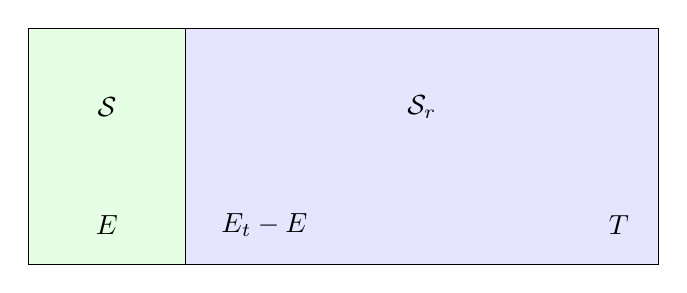
\begin{tikzpicture}
		\fill[blue!10!white] (0,0) rectangle (8,3);
		\draw (0,0) rectangle (8,3);
		\fill[green!10!white] (0,0) rectangle (2,3);
		\draw (0,0) rectangle (2,3);
		\node at (1,2) {$\mathcal{S}$};
		\node at (1,0.5) {$E$};
		\node at (5,2) {$\mathcal{S}_r$};
		\node at (7.5,0.5) {$T$};
		\node at (3,0.5) {$E_t - E$};
	\end{tikzpicture}
\end{center}

Considere que os sistemas estão em contato térmico e o sistema completo, junto com o banho é um sistema isolado de energia $E_t$. Sabemos que a probabilidade de uma energia no nosso sistema termalizado ($\rho_E$) é expressa:

\[
	\rho_E = \sum_{\sigma} \rho_\sigma = \Omega(E)\rho_\sigma
\]

Onde note, $\rho_\sigma$ é a probabilidade de, dada uma temperatura, um microestado possível. Note por outro lado que podemos expressar:

\[
	\rho_E = \frac{\Omega(E) \Omega_r (E_t - E)}{\sum_{i} \Omega(E_i) \Omega_r(E_t-E)}
\]

Note que isso é nada mais do que dizer que os microestados são equiprováveis e basta uma contagem (normalizada) para definir a probabilidade. Neste sentido podemos também escrever:

\[
	\rho_\sigma \propto \Omega_r(E_t - E)
\]

Isso é, quanto mais formas o reservatório possa se organizar para determinada energia, mais provável é o microestado associado à energia de $\mathcal{S}$.

\begin{align*}
	\rho_\sigma & \propto e^{\beta T K_b \log{(\Omega_r(E_t - E))}} \\
				& \propto e^{\beta T \left( \mathcal{S}_r(E_t) - \frac{E}{T}\right) } \\
				& \propto e^{-\beta E} e^{\beta T \mathcal{S}_r(E_t)} \\
				& \propto e^{-\beta E}
\end{align*}

Onde fizemos a expansão de $k_b \log{(\Omega_r(E_t - E))}$ (entropia) em Taylor (apesar de que, em realidade, apenas $\frac{E}{E_t}$ é pequeno, não necessariamente $E$) e obtemos

\[
	\mathcal{S}_r(E_t - E) \approx \mathcal{S}_r(E_t) + \left( \frac{\partial \mathcal{S}_r}{\partial E}\right)_{E=E_t} (-E)
\]

Onde 

\[
	\left( \frac{\partial \mathcal{S}_r}{\partial E} \right)_{E=E_t} = \frac{1}{T}
\]

\subsection{A entropia de Shannon}

Podemos fazer algo um pouco mais matemático. Definiremos a entropia de Shannon

\[
	\mathcal{S} = -k_b \sum_{i} p_i \log{p_i}
\]

\subsubsection{Um vínculo}

Se impormos um vínculo do tipo

\[
	\sum_{i} p_i = 1
\]

Podemos usar os multiplicadores de Lagrange para realizar a maximização da nossa função. Pela definição, escrevemos:

\[
	S({p_i}, \lambda) \equiv k_b \sum_{i=1}^{N} p_i \log{(p_i)} - \lambda \left( \sum_{i=1}^{N}p_i -1 \right) 
\]

Com diferencial

\[
	\delta S = - k_b \sum_{i=1}^{N} \left( p_i \log{p_i} + \frac{p_i}{p_i} \delta p_i \right) - \lambda \sum_{i=1}^{N}\delta p_i
\]

Resolveremos agora o sistema

\[
 \begin{cases}
	\delta S = 0 \\
	\sum_{i} p_i = 1
\end{cases}
\]

ou seja,

\[
\begin{cases}
	-k_b (\log{p_i} + 1) - \lambda \\
	\sum_{i} p_i = 1
\end{cases}
\]

Note que $p_i = cte \ \forall i$. Teremos então $p_i = \frac{1}{N}$. A entropia neste caso será 

\[
	S({p_i}^*) = - k_b \sum_{i=1}^{N} \left( \frac{1}{N} \log{\frac{1}{N}} \right) = k_b \log{N}
\]

\subsubsection{Dois vínculos}

Faremos agora a implicação de um novo vínculo

\[
\sum_{\sigma} p_\sigma E_\sigma = U
\]

Desenvolvendo a equação

\[
S({p_i}, \lambda) \equiv k_b \sum_{i=1}^{N} p_i \log{(p_i)} - \lambda_1 \left( \sum_{i=1}^{N}p_i -1 \right)  - \lambda_2 \left( \sum_\sigma  p_\sigma E_\sigma - U \right) 
\]

Chegaremos no sistema


\[
\begin{cases}
	-k_b (\log{p_i} + 1) - \lambda_1 - \lambda_2 E_\sigma \\
	\sum_{\sigma} p_i = 1 \\
	\sum_{\sigma} p_\sigma E_\sigma = U
\end{cases}
\]

E finalmente, da primeira equação tiramos

\[
	p_\sigma = e^{A E_\sigma + B} = M e^{-\beta E_\sigma}
\]

De forma que podemos reescrever

\[
	1 = \sum_\sigma M e^{-\beta E_\sigma} = M \sum_\sigma e^{-\beta E_\sigma}
\]

Onde nomearemos $M = \frac{1}{\sum_{\sigma}e^{-\beta E_\sigma}} = \frac{1}{\mathcal{Z}}$ \textbf{função partição}. Falta apenas definir $\beta$ em

\[
	p_\sigma = \frac{e^{-\beta E_\sigma}}{Z}
\]

Para $\beta$ podemos aplicar o último vínculo (da temperatura térmica)

\[
	U = \sum_\sigma p_\sigma E_\sigma = \sum_\sigma \left( \frac{1}{Z} e^{-\beta E_\sigma} \right) E_\sigma = \frac{1}{Z} \sum_\sigma E_\sigma e^{-\beta E_\sigma}
\]

\[
	-\frac{1}{Z} \frac{\partial }{ \partial \beta} \left( \sum_\sigma e^{-\beta E_\sigma} \right) = -\frac{1}{\mathcal{Z}} \frac{\partial Z}{\partial \beta} = - \frac{\partial (\log{Z})}{\partial \beta}
\]

De alguma forma esta equação transcendental nos define $\beta$.

\subsection{Conexão Micro-Macro}

Quando tratamos destes sistemas no ensemble canônico a energia interna não mais será minimizada no nosso sistema termalizado. Introduzimos uma nova grandeza chamada Energia Livre de Helmholtz ($F$), definida como a transformada de Legendre (discutida no Apêndice \ref{apdx: legendre}) da energia interna em relação à entropia, ou seja

\begin{equation}
	 U(S,V,N) \mapsto F(T, V, N)
\end{equation}

ou ainda mais especificamente

\[
	F(T, V, N) = U(S(T,V,N), V, N) - T S(T,V,N) 
\]

Note ainda as diferenciais

\begin{align*}
	& dU = TdS - PdV + \mu dN \\
	& dF = -SdT - PdV + \mu dN
\end{align*}

Um sistema termalizado vai querer minimizar essa nova grandeza da energia livre de Helmholtz. Em todo caso iniciaremos com a expressão já deduzida da euqação de partição

\[
	\mathcal{Z} = \sum_{\sigma} e^{-\beta E_\sigma}
\]

Que pode ser reescrito em termos de uma soma na energia

\begin{align*}
	& \mathcal{Z} = \sum_{E} e^{-\beta E} \Omega(E) \\
	& \mathcal{Z} = \sum_{E} e^{-\beta T K_b \log{(\Omega(E))}} \Omega(E)
\end{align*}

Podemos argumentar que $ K_b \log{(\Omega(E))} = S(E)$ e usaremos o logaritmo de somas assintóticas (discutido no Apêndice \ref{apdx: somaassin}) para terminar o desenvolvimento. Note

\begin{align*}
	& \log{(\mathcal{Z})} \approx \log{\left( \max_x{[e^{-\beta(E - T S(E))}]} \right)} \\
	& \log{(\mathcal{Z})} \approx \log{\left(e^{-\beta \min_E{((E - T S(E)))}} \right)}
\end{align*}

Onde podemos reconhecer pela transformada de Legendre o termo referente à Energia livre de Helmholtz. Tendo assim

\[
	\log{(\mathcal{Z})} \approx -\beta F
\]	

\begin{equation}
	F = - K_b T \log{(\mathcal{Z})}
\end{equation}
